\chapter{R\'{e}alisation}
\label{chap:realisation}

\vspace{2cm}

\noindent\textbf{\Large Plan}

\vspace{0.5cm}
\noindent\rule{\textwidth}{0.4pt}
\vspace{0.3cm}

\begin{list}{}{\setlength{\leftmargin}{1.5cm}\setlength{\itemsep}{6pt}}
  \item \textbf{1} \hspace{0.3cm} Environnement de travail \dotfill \pageref{sec:env}
  \item \textbf{2} \hspace{0.3cm} R\'{e}alisation des sprints \dotfill \pageref{sec:sprints}
  \item \textbf{3} \hspace{0.3cm} Tests et qualit\'{e} \dotfill \pageref{sec:tests}
  \item \textbf{4} \hspace{0.3cm} Conclusion \dotfill \pageref{sec:concl3}
\end{list}

\vspace{0.3cm}
\noindent\rule{\textwidth}{0.4pt}

\newpage

\section*{Introduction}

Ce chapitre pr\'{e}sente la mise en \oe uvre concr\`{e}te du syst\`{e}me AutoAssist. Apr\`{e}s avoir d\'{e}fini l'environnement mat\'{e}riel et logiciel dans lequel le projet a \'{e}t\'{e} d\'{e}velopp\'{e}, nous d\'{e}taillons la r\'{e}alisation de chacun des six sprints en illustrant les r\'{e}sultats par des captures d'\'{e}cran et des diagrammes. Pour chaque sprint, nous pr\'{e}sentons les choix d'impl\'{e}mentation, les difficult\'{e}s rencontr\'{e}es et les solutions adopt\'{e}es. Enfin, nous exposons la strat\'{e}gie de test et les outils de qualit\'{e} int\'{e}gr\'{e}s au pipeline de livraison continue.


% ╔══════════════════════════════════════════════════════════════╗
%                SECTION 1 : ENVIRONNEMENT DE TRAVAIL
% ╚══════════════════════════════════════════════════════════════╝
\section{Environnement de travail}
\label{sec:env}

\subsection{Environnement mat\'{e}riel}

Le d\'{e}veloppement a \'{e}t\'{e} r\'{e}alis\'{e} sur la machine suivante~:

\begin{table}[H]
\centering
\caption{Configuration mat\'{e}rielle}
\label{tab:materiel}
\begin{tabular}{|p{4cm}|p{8cm}|}
\hline
\textbf{Composant} & \textbf{Sp\'{e}cification} \\
\hline
Ordinateur & HP ZBook \\
\hline
Processeur & Intel Core i7 \\
\hline
M\'{e}moire vive & 16 Go RAM \\
\hline
Stockage & SSD 512 Go \\
\hline
Syst\`{e}me d'exploitation & Windows 11 \\
\hline
\end{tabular}
\end{table}

\subsection{Environnement logiciel}

Cette sous-section pr\'{e}sente de mani\`{e}re d\'{e}taill\'{e}e l'ensemble des technologies, frameworks, bases de donn\'{e}es et outils utilis\'{e}s tout au long du d\'{e}veloppement de la plateforme AutoAssist.

\subsubsection{Langages de programmation}

Le tableau~\ref{tab:langages} r\'{e}capitule les langages utilis\'{e}s dans le projet. Le choix de combiner Java, Python, JavaScript/TypeScript et Dart r\'{e}pond \`{a} la n\'{e}cessit\'{e} d'adresser des domaines m\'{e}tier diff\'{e}rents (backend transactionnel, intelligence artificielle, frontend r\'{e}actif et application mobile).

\begin{table}[H]
\centering
\caption{Langages de programmation utilis\'{e}s}
\label{tab:langages}
\begin{tabular}{|p{3.5cm}|p{2cm}|p{7.5cm}|}
\hline
\textbf{Langage} & \textbf{Version} & \textbf{Utilisation} \\
\hline
Java (JDK) & 21 & Backend principal -- 7 microservices Spring Boot \\
\hline
Python & 3.11 & Service IA (FastAPI, Whisper, spaCy, RAG) \\
\hline
JavaScript (Node.js) & 20 & Service WhatsApp (chatbot, gestion de groupes) \\
\hline
TypeScript & 5.x & Typage statique du frontend React \\
\hline
Dart & 3.x & Application mobile Flutter \\
\hline
SQL & -- & Requ\^{e}tes PostgreSQL, migrations, agr\'{e}gations \\
\hline
\end{tabular}
\end{table}

\subsubsection{Frameworks et librairies}

Le tableau~\ref{tab:frameworks} pr\'{e}sente les frameworks et librairies cl\'{e}s du projet.

\begin{longtable}{|p{3.5cm}|p{2cm}|p{7.5cm}|}
\caption{Frameworks et librairies utilis\'{e}s} \label{tab:frameworks} \\
\hline
\textbf{Framework / Librairie} & \textbf{Version} & \textbf{Utilisation} \\
\hline
\endfirsthead
\hline \textbf{Framework / Librairie} & \textbf{Version} & \textbf{Utilisation} \\ \hline
\endhead
Spring Boot \cite{springboot} & 3.3 & Framework backend (REST, JPA, Security, Mail) \\
\hline
Spring Cloud & 2024.0 & Eureka Discovery, Gateway, OpenFeign \\
\hline
Resilience4j & 2.x & Circuit Breaker pour le LLM (fallback automatique) \\
\hline
FastAPI & 0.110 & API REST asynchrone du service IA (Python) \\
\hline
React & 18 & Frontend web SPA (12 pages, 9 services API) \\
\hline
Vite & 5.x & Bundler rapide du frontend React \\
\hline
Flutter \cite{flutter} & 3.x & Application mobile multiplateforme (11 \'{e}crans) \\
\hline
whatsapp-web.js & 1.x & Chatbot WhatsApp (Node.js + Puppeteer) \\
\hline
OpenAI Whisper & small & Transcription audio automatique (STT) \\
\hline
spaCy & 3.x & Analyse NLP (\texttt{fr\_core\_news\_sm}) \\
\hline
ChromaDB & 0.4 & Base de donn\'{e}es vectorielle pour le RAG \\
\hline
SentenceTransformers & 2.x & Embeddings multilingues (MiniLM-L12-v2) \\
\hline
Thymeleaf & 3.x & Moteur de templates emails HTML \\
\hline
Axios / Dio & -- & Clients HTTP (React / Flutter) avec interceptors JWT \\
\hline
fl\_chart & 0.x & Graphiques analytiques dans Flutter \\
\hline
\end{longtable}

\subsubsection{Biblioth\`{e}ques et packages}

Le tableau~\ref{tab:packages} pr\'{e}sente les biblioth\`{e}ques et packages sp\'{e}cifiques utilis\'{e}s dans le projet, qui jouent un r\^{o}le essentiel dans le d\'{e}veloppement et la gestion des donn\'{e}es.

\begin{longtable}{|p{4cm}|p{2cm}|p{6.5cm}|}
\caption{Biblioth\`{e}ques et packages importants} \label{tab:packages} \\
\hline
\textbf{Package} & \textbf{Plateforme} & \textbf{Utilisation} \\
\hline
\endfirsthead
\hline \textbf{Package} & \textbf{Plateforme} & \textbf{Utilisation} \\ \hline
\endhead
spring-boot-starter-data-jpa & Maven & ORM JPA/Hibernate pour PostgreSQL \\
\hline
spring-cloud-starter-openfeign & Maven & Communication synchrone inter-services \\
\hline
iText PDF & Maven & G\'{e}n\'{e}ration de courriers PDF (d\'{e}cisions) \\
\hline
hypersistence-utils & Maven & Support JSONB natif pour PostgreSQL \\
\hline
rouge-score & pip & Calcul de la m\'{e}trique ROUGE-1 pour l'\'{e}valuation RAG \\
\hline
sentence-transformers & pip & Embeddings multilingues (MiniLM-L12-v2) \\
\hline
uvicorn & pip & Serveur ASGI pour FastAPI \\
\hline
pydub & pip & Manipulation audio (conversion, d\'{e}coupage) \\
\hline
react-router-dom & npm & Routage SPA avec guards RBAC \\
\hline
recharts & npm & Graphiques interactifs (dashboard, analytics) \\
\hline
stompjs / sockjs-client & npm & WebSocket STOMP pour notifications temps r\'{e}el \\
\hline
puppeteer & npm & Navigateur headless pour whatsapp-web.js \\
\hline
provider & pub.dev & Gestion d'\'{e}tat r\'{e}active dans Flutter \\
\hline
dio & pub.dev & Client HTTP avec interceptors JWT (Flutter) \\
\hline
\end{longtable}

\subsubsection{Bases de donn\'{e}es et middleware}

Le syst\`{e}me AutoAssist utilise neuf bases de donn\'{e}es PostgreSQL isol\'{e}es (une par microservice), une base de donn\'{e}es vectorielle et deux services de middleware.

\begin{table}[H]
\centering
\caption{Bases de donn\'{e}es et middleware}
\label{tab:bdd_middleware}
\begin{tabular}{|p{3.5cm}|p{2cm}|p{7.5cm}|}
\hline
\textbf{Technologie} & \textbf{Version} & \textbf{Utilisation} \\
\hline
PostgreSQL & 15-alpine & 9 bases isol\'{e}es (auth, users, tickets, rules, decisions, notif, analytics, ai, n8n) \\
\hline
pgvector & 0.7 & Extension vectorielle pour les embeddings RAG \\
\hline
Redis & 7-alpine & Cache des d\'{e}cisions (SHA-256, TTL 1h), rate limiting \\
\hline
RabbitMQ & 3-management & Bus \'{e}v\'{e}nementiel asynchrone (4 exchanges, 7 events, 10+ queues) \\
\hline
ChromaDB & 0.4 & Stockage vectoriel pour la recherche s\'{e}mantique RAG \\
\hline
\end{tabular}
\end{table}

\subsubsection{Outils DevOps et d\'{e}ploiement}

\begin{table}[H]
\centering
\caption{Outils DevOps}
\label{tab:devops}
\begin{tabular}{|p{3.5cm}|p{2cm}|p{7.5cm}|}
\hline
\textbf{Outil} & \textbf{Version} & \textbf{Utilisation} \\
\hline
Docker & 27+ & Conteneurisation (17 conteneurs) \\
\hline
Docker Compose & 2.x & Orchestration locale avec healthchecks \\
\hline
Jenkins & 2.x & Pipeline CI/CD (9 \'{e}tapes automatis\'{e}es) \\
\hline
SonarCloud & -- & Analyse statique et qualit\'{e} du code \\
\hline
n8n & 1.x & Automatisation (8 workflows : alertes, rapports, backups) \\
\hline
Nginx & 1.25 & Reverse proxy, CORS, WebSocket upgrade \\
\hline
Git / GitHub & -- & Gestion de version et collaboration \\
\hline
\end{tabular}
\end{table}

\subsubsection{Environnements de d\'{e}veloppement (IDEs)}

\begin{table}[H]
\centering
\caption{Environnements de d\'{e}veloppement}
\label{tab:ides}
\begin{tabular}{|p{3.5cm}|p{2cm}|p{7.5cm}|}
\hline
\textbf{IDE} & \textbf{Version} & \textbf{Utilisation} \\
\hline
IntelliJ IDEA & 2024 & D\'{e}veloppement Java / Spring Boot \\
\hline
VS Code & 1.90+ & D\'{e}veloppement Python, React, Flutter \\
\hline
Postman & 11 & Tests manuels des API REST \\
\hline
DBeaver & 24 & Administration et requ\^{e}tes PostgreSQL \\
\hline
\end{tabular}
\end{table}


% ╔══════════════════════════════════════════════════════════════╗
%                SECTION 2 : REALISATION DES SPRINTS
% ╚══════════════════════════════════════════════════════════════╝
\section{R\'{e}alisation des sprints}
\label{sec:sprints}

Cette section d\'{e}taille la r\'{e}alisation de chaque sprint, en pr\'{e}sentant les fonctionnalit\'{e}s d\'{e}velopp\'{e}es, les choix techniques et les r\'{e}sultats obtenus.

% ══════════════════════════════════════
% SPRINT 1
% ══════════════════════════════════════
\subsection{Sprint 1~: Infrastructure, CI/CD et authentification}

\subsubsection{Mise en place de l'infrastructure Docker}

L'infrastructure du syst\`{e}me AutoAssist repose sur 17 conteneurs Docker orchestr\'{e}s via Docker Compose (469 lignes de configuration). Chaque microservice dispose de son propre conteneur, de sa propre base de donn\'{e}es et de son propre healthcheck. L'ordre de d\'{e}marrage respecte les d\'{e}pendances~: les services d'infrastructure (PostgreSQL, Redis, RabbitMQ) d\'{e}marrent en premier, suivis d'Eureka Server, de l'API Gateway, puis des services m\'{e}tier. Un r\'{e}seau Docker d\'{e}di\'{e} (\texttt{callmgmt-net}) assure l'isolation et la communication entre les conteneurs.

\begin{figure}[H]
    \centering
    % \includegraphics[width=0.95\textwidth]{figures/docker_ps.png}
    \fbox{\parbox{0.9\textwidth}{\centering\vspace{2cm}\textit{[Capture -- docker ps montrant les 17 conteneurs]}\vspace{2cm}}}
    \caption{Les 17 conteneurs Docker du syst\`{e}me AutoAssist}
    \label{fig:docker_ps}
\end{figure}

\subsubsection{Pipeline CI/CD Jenkins}

Un pipeline Jenkins d\'{e}claratif complet a \'{e}t\'{e} mis en place avec 9 \'{e}tapes automatis\'{e}es~: Checkout, Build \& Test (parall\`{e}le Java + Python + Frontend), SonarCloud Analysis, Docker Build, Registry Push, Deploy Staging, Smoke Tests, Database Backup et Notification. Le pipeline int\`{e}gre un backup automatique de la base de donn\'{e}es avant chaque d\'{e}ploiement et envoie une notification par email en cas d'\'{e}chec.

\begin{figure}[H]
    \centering
    % \includegraphics[width=0.95\textwidth]{figures/jenkins_pipeline.png}
    \fbox{\parbox{0.9\textwidth}{\centering\vspace{2.5cm}\textit{[Capture -- Pipeline Jenkins avec les 9 \'{e}tapes]}\vspace{2.5cm}}}
    \caption{Pipeline CI/CD Jenkins -- vue d'ensemble}
    \label{fig:jenkins}
\end{figure}

\subsubsection{Authentification JWT et RBAC}

Le service d'authentification impl\'{e}mente un syst\`{e}me JWT complet avec access token (contenant userId, email, role et agenceId) et refresh token (persist\'{e} en base, r\'{e}vocable). Le contr\^{o}le d'acc\`{e}s RBAC distingue trois r\^{o}les~: \textbf{Administrateur} (gestion globale), \textbf{Superviseur} (validation des d\'{e}cisions, r\`{e}gles) et \textbf{Op\'{e}rateur} (traitement des tickets). Les mots de passe sont hach\'{e}s via BCrypt et le refresh token supporte la rotation automatique.

L'interface de connexion, pr\'{e}sent\'{e}e dans la figure~\ref{fig:login}, assure l'authentification s\'{e}curis\'{e}e des utilisateurs. L'\'{e}cran affiche un formulaire avec les champs email et mot de passe. Si les identifiants sont valides, l'utilisateur est redirig\'{e} vers le tableau de bord correspondant \`{a} son r\^{o}le~; sinon, un message d'erreur s'affiche pour l'inviter \`{a} corriger sa saisie.

\begin{figure}[H]
    \centering
    % \includegraphics[width=0.85\textwidth]{figures/login_page.png}
    \fbox{\parbox{0.8\textwidth}{\centering\vspace{2.5cm}\textit{[Capture -- Page de connexion AutoAssist]}\vspace{2.5cm}}}
    \caption{Interface de connexion avec authentification JWT}
    \label{fig:login}
\end{figure}

\subsubsection{Service Discovery et API Gateway}

Eureka Server assure la d\'{e}couverte automatique des services au d\'{e}marrage. L'API Gateway Spring Cloud expose 12 routes prot\'{e}g\'{e}es par trois filtres en cascade~: \texttt{JwtAuthFilter} (validation du token), \texttt{RoleFilter} (v\'{e}rification du r\^{o}le RBAC) et \texttt{RateLimiterFilter} (limitation \`{a} 100 requ\^{e}tes par seconde par IP via Redis). La Gateway g\`{e}re \'{e}galement la politique CORS et le WebSocket upgrade pour les notifications temps r\'{e}el.

\begin{figure}[H]
    \centering
    % \includegraphics[width=0.85\textwidth]{figures/eureka_dashboard.png}
    \fbox{\parbox{0.8\textwidth}{\centering\vspace{2cm}\textit{[Capture -- Dashboard Eureka avec les services enregistr\'{e}s]}\vspace{2cm}}}
    \caption{Dashboard Eureka -- services enregistr\'{e}s}
    \label{fig:eureka}
\end{figure}


% ══════════════════════════════════════
% SPRINT 2
% ══════════════════════════════════════
\subsection{Sprint 2~: Gestion des organisations et des tickets}

\subsubsection{Gestion des utilisateurs et agences}

Le module d'organisation permet la gestion compl\`{e}te des utilisateurs (CRUD, attribution des r\^{o}les RBAC, activation/d\'{e}sactivation) et des agences (cr\'{e}ation, assignation d'un responsable). Lors de la cr\'{e}ation d'une agence, un \'{e}v\'{e}nement RabbitMQ \texttt{agence.created} est publi\'{e}, d\'{e}clenchant automatiquement la cr\'{e}ation d'un groupe WhatsApp d\'{e}di\'{e} dans le service de messagerie.

L'interface de gestion des utilisateurs, pr\'{e}sent\'{e}e dans la figure~\ref{fig:users}, permet \`{a} l'administrateur de consulter la liste compl\`{e}te des utilisateurs enregistr\'{e}s, de modifier leurs informations personnelles, d'attribuer ou de changer leurs r\^{o}les (Administrateur, Superviseur, Op\'{e}rateur), et de d\'{e}sactiver un compte. La suppression est s\'{e}curis\'{e}e par une confirmation pr\'{e}alable pour \'{e}viter toute action accidentelle.

\begin{figure}[H]
    \centering
    % \includegraphics[width=0.95\textwidth]{figures/users_page.png}
    \fbox{\parbox{0.9\textwidth}{\centering\vspace{2.5cm}\textit{[Capture -- Page de gestion des utilisateurs]}\vspace{2.5cm}}}
    \caption{Interface de gestion des utilisateurs (RBAC)}
    \label{fig:users}
\end{figure}

L'interface de gestion des agences, illustr\'{e}e par la figure~\ref{fig:agences}, permet \`{a} l'administrateur de cr\'{e}er de nouvelles agences, d'y assigner un responsable et de consulter les informations de chaque agence (nom, adresse, responsable, num\'{e}ro de t\'{e}l\'{e}phone). Lors de la cr\'{e}ation, le syst\`{e}me d\'{e}clenche automatiquement la cr\'{e}ation d'un groupe WhatsApp d\'{e}di\'{e} \`{a} l'agence.

\begin{figure}[H]
    \centering
    % \includegraphics[width=0.95\textwidth]{figures/agences_page.png}
    \fbox{\parbox{0.9\textwidth}{\centering\vspace{2.5cm}\textit{[Capture -- Page de gestion des agences]}\vspace{2.5cm}}}
    \caption{Interface de gestion des agences}
    \label{fig:agences}
\end{figure}

\subsubsection{Gestion des tickets multicanaux}

Le syst\`{e}me de tickets supporte trois canaux d'acquisition distincts, chacun impl\'{e}ment\'{e} via un contr\^{o}leur d\'{e}di\'{e} dans le \texttt{ChannelAcquisitionController}~:

\begin{itemize}
    \item \textbf{Canal CALL (Twilio VoIP)} -- Le contr\^{o}leur \texttt{TwilioWebhookController} (286 lignes) expose quatre webhooks~: \texttt{/voice} (menu IVR TwiML avec consentement), \texttt{/recording} (r\'{e}ception de l'URL audio), \texttt{/recording-done} (d\'{e}clenchement du pipeline IA) et \texttt{/status} (\'{e}v\'{e}nements d'appel). La signature Twilio est valid\'{e}e via \texttt{RequestValidator} pour garantir l'authenticit\'{e} des requ\^{e}tes.
    \item \textbf{Canal EMAIL (IMAP)} -- Le service \texttt{EmailListenerService} (313 lignes) interroge le serveur IMAP toutes les 30 secondes (\texttt{@Scheduled(fixedRate=30000)}). Les emails sont filtr\'{e}s par mots-cl\'{e}s m\'{e}tier (\og r\'{e}clamation \fg, \og panne \fg, \og sinistre \fg) et un m\'{e}canisme anti-boucle ignore les messages provenant de l'adresse syst\`{e}me.
    \item \textbf{Canal WEB (formulaire public)} -- Un formulaire accessible sans authentification permet aux clients de soumettre une demande avec consentement explicite (checkbox). Le ticket est cr\'{e}\'{e} directement en file d'attente.
\end{itemize}

Chaque ticket re\c{c}oit un num\'{e}ro unique au format \texttt{T-YYYYMMDD-XXXX} et suit un cycle de vie complet~: NOUVEAU $\rightarrow$ EN\_COURS $\rightarrow$ RESOLU $\rightarrow$ FERME. La transition entre les statuts est valid\'{e}e par la m\'{e}thode \texttt{canTransitionTo()} et chaque changement est trac\'{e} dans un audit trail (\texttt{TicketAction}). Le syst\`{e}me supporte \'{e}galement l'upload de photos de sinistre (multi-fichiers, validation MIME \texttt{image/*}, taille max 10 Mo par fichier) stock\'{e}es en format JSONB et servies avec un cache de 24 heures.

L'interface de gestion des tickets, pr\'{e}sent\'{e}e dans la figure~\ref{fig:tickets}, permet aux op\'{e}rateurs de consulter l'ensemble des tickets avec un syst\`{e}me de filtrage avanc\'{e} par statut (Nouveau, En cours, R\'{e}solu, Ferm\'{e}), par canal d'acquisition (Appel, Email, Web) et par priorit\'{e}. Un clic sur un ticket ouvre sa page de d\'{e}tail compl\`{e}te, incluant la transcription audio, l'analyse NLP, l'historique des actions et la d\'{e}cision associ\'{e}e.

\begin{figure}[H]
    \centering
    % \includegraphics[width=0.95\textwidth]{figures/ticket_list.png}
    \fbox{\parbox{0.9\textwidth}{\centering\vspace{2.5cm}\textit{[Capture -- Liste des tickets avec filtres]}\vspace{2.5cm}}}
    \caption{Liste des tickets avec filtrage par statut et canal}
    \label{fig:tickets}
\end{figure}

\subsubsection{Softphone web int\'{e}gr\'{e}}

Pour les appels en interne, un softphone web (606 lignes) est int\'{e}gr\'{e} directement au service IA. Son interface glassmorphism inclut un visualiseur audio FFT en temps r\'{e}el. Le softphone utilise l'API \texttt{MediaRecorder} du navigateur (format WebM/Opus, 16 kHz, mono) et ex\'{e}cute le pipeline complet de mani\`{e}re transparente~: enregistrement $\rightarrow$ cr\'{e}ation du ticket CALL $\rightarrow$ upload de l'audio $\rightarrow$ transcription Whisper $\rightarrow$ analyse NLP.

\begin{figure}[H]
    \centering
    % \includegraphics[width=0.85\textwidth]{figures/softphone.png}
    \fbox{\parbox{0.8\textwidth}{\centering\vspace{2.5cm}\textit{[Capture -- Softphone web avec visualiseur audio]}\vspace{2.5cm}}}
    \caption{Softphone web -- enregistrement et visualiseur audio FFT}
    \label{fig:softphone}
\end{figure}

\subsubsection{Formulaire public et file d'attente}

Le formulaire public permet aux clients de soumettre une demande sans authentification. Les tickets cr\'{e}\'{e}s par les canaux EMAIL et WEB sont plac\'{e}s dans une file d'attente tri\'{e}e par priorit\'{e} (ASC) puis par date de cr\'{e}ation (FIFO). Les op\'{e}rateurs peuvent prendre un ticket depuis la file, d\'{e}clenchant automatiquement la transition de statut NOUVEAU $\rightarrow$ EN\_COURS.

\begin{figure}[H]
    \centering
    % \includegraphics[width=0.85\textwidth]{figures/public_form.png}
    \fbox{\parbox{0.8\textwidth}{\centering\vspace{2.5cm}\textit{[Capture -- Formulaire public de soumission]}\vspace{2.5cm}}}
    \caption{Formulaire public de soumission de demande (canal WEB)}
    \label{fig:public_form}
\end{figure}


% ══════════════════════════════════════
% SPRINT 3
% ══════════════════════════════════════
\subsection{Sprint 3~: Service IA et d\'{e}veloppement frontend}

\subsubsection{Transcription audio avec Whisper}

Le service IA (Python FastAPI) int\`{e}gre le mod\`{e}le OpenAI Whisper (variante \texttt{small}) pour la transcription automatique des enregistrements audio en fran\c{c}ais. Le processus g\'{e}n\`{e}re le texte transcrit, les segments temporels avec horodatage, un score de confiance calcul\'{e} \`{a} partir de la moyenne logarithmique des probabilit\'{e}s ($1 + \text{avg\_logprob}$) et la dur\'{e}e totale de l'audio. Les formats accept\'{e}s sont~: WAV, MP3, OGG, MP4, WebM, FLAC, M4A et AAC, avec une taille maximale de 50 Mo.

\begin{figure}[H]
    \centering
    % \includegraphics[width=0.95\textwidth]{figures/transcription.png}
    \fbox{\parbox{0.9\textwidth}{\centering\vspace{2.5cm}\textit{[Capture -- Transcription audio dans le d\'{e}tail du ticket]}\vspace{2.5cm}}}
    \caption{R\'{e}sultat de la transcription Whisper dans le d\'{e}tail du ticket}
    \label{fig:transcription}
\end{figure}

\subsubsection{Transcription en streaming via WebSocket}

En compl\'{e}ment de la transcription par fichier, un mode streaming temps r\'{e}el a \'{e}t\'{e} impl\'{e}ment\'{e} via WebSocket (\texttt{/ws/transcribe/\{ticket\_id\}}). Le client envoie des chunks audio binaires en continu~; le serveur renvoie des r\'{e}sultats partiels (\texttt{\{type: "partial", text, elapsed\}}) puis un r\'{e}sultat final (\texttt{\{type: "final", text, duration\}}). Le buffer accumule entre 48 Ko ($\approx$ 3 secondes) et 960 Ko ($\approx$ 30 secondes) d'audio avant de lancer une transcription partielle, offrant ainsi un retour visuel quasi instantan\'{e} \`{a} l'op\'{e}rateur pendant l'appel.

\subsubsection{Analyse NLP avec spaCy}

L'analyse NLP locale utilise le mod\`{e}le spaCy \texttt{fr\_core\_news\_sm} et des heuristiques linguistiques pour extraire automatiquement quatre types d'informations~:

\begin{itemize}
    \item \textbf{R\'{e}f\'{e}rence pi\`{e}ce}~: regex \texttt{[A-Z]\{2,4\}-\textbackslash d\{4,8\}} combin\'{e} avec un dictionnaire de 20 mots-cl\'{e}s m\'{e}caniques.
    \item \textbf{Type de sinistre}~: classification en 5 cat\'{e}gories (PANNE, ACCIDENT, USURE, D\'{E}FAUT\_FABRICATION, VOL) par correspondance de mots-cl\'{e}s pond\'{e}r\'{e}s.
    \item \textbf{Sentiment client}~: POSITIF, N\'{E}GATIF ou NEUTRE par analyse d'expressions et de fronti\`{e}res lexicales.
    \item \textbf{Mots-cl\'{e}s}~: extraction des entit\'{e}s nomm\'{e}es (LOC, ORG, MISC, PER) et lemmatisation des noms, top 10.
\end{itemize}

Le score de confiance est de 0.9 si la pi\`{e}ce et le sinistre sont d\'{e}tect\'{e}s, 0.6 sinon. Ces donn\'{e}es pr\'{e}-remplissent automatiquement le formulaire de d\'{e}cision.

\begin{figure}[H]
    \centering
    % \includegraphics[width=0.95\textwidth]{figures/nlp_analysis.png}
    \fbox{\parbox{0.9\textwidth}{\centering\vspace{2.5cm}\textit{[Capture -- R\'{e}sultat analyse NLP : sinistre, sentiment, mots-cl\'{e}s]}\vspace{2.5cm}}}
    \caption{R\'{e}sultat de l'analyse NLP (spaCy) -- extraction automatique}
    \label{fig:nlp}
\end{figure}

\subsubsection{Tableau de bord principal et notifications temps r\'{e}el}

Le dashboard React offre une vue synth\'{e}tique de l'activit\'{e}~: nombre total de tickets, taux de r\'{e}solution, temps de traitement moyen, r\'{e}partition par canal et par statut, ainsi que les derniers tickets cr\'{e}\'{e}s.

Les mises \`{a} jour du tableau de bord sont pouss\'{e}es en \textbf{temps r\'{e}el via le protocole WebSocket STOMP}. Le ticket-service publie des messages sur deux topics d\'{e}di\'{e}s~:
\begin{itemize}
    \item \texttt{/topic/tickets.new} -- notifie instantan\'{e}ment tous les op\'{e}rateurs connect\'{e}s de la cr\'{e}ation d'un nouveau ticket.
    \item \texttt{/topic/tickets.update} -- diffuse les changements de statut et d'assignation en temps r\'{e}el.
\end{itemize}
C\^{o}t\'{e} client, la biblioth\`{e}que \texttt{stompjs} (avec \texttt{sockjs-client} comme fallback) \'{e}tablit une connexion persistante via l'API Gateway, qui g\`{e}re le WebSocket upgrade. Cette architecture \'{e}v\'{e}nementielle \'{e}limine le besoin de polling et garantit une r\'{e}activit\'{e} optimale de l'interface.

\begin{figure}[H]
    \centering
    % \includegraphics[width=0.95\textwidth]{figures/dashboard.png}
    \fbox{\parbox{0.9\textwidth}{\centering\vspace{2.5cm}\textit{[Capture -- Dashboard principal avec KPIs et graphiques]}\vspace{2.5cm}}}
    \caption{Tableau de bord principal -- KPIs et statistiques en temps r\'{e}el}
    \label{fig:dashboard}
\end{figure}

\subsubsection{Page de d\'{e}tail du ticket}

La page de d\'{e}tail du ticket (\texttt{TicketDetailPage}, 992 lignes, 51 Ko) constitue l'interface la plus riche du syst\`{e}me. Comme l'illustre la figure~\ref{fig:ticket_detail}, elle centralise l'ensemble des informations et des actions relatives \`{a} un ticket en une vue unifi\'{e}e~:

\begin{itemize}
    \item \textbf{Informations g\'{e}n\'{e}rales}~: num\'{e}ro du ticket, canal d'acquisition, statut actuel, priorit\'{e}, nom et coordonn\'{e}es du client, op\'{e}rateur assign\'{e}, horodatage de cr\'{e}ation.
    \item \textbf{Transcription audio en direct}~: pour les tickets CALL, la transcription Whisper s'affiche en temps r\'{e}el via le flux WebSocket, avec un indicateur de progression et un score de confiance.
    \item \textbf{R\'{e}sultat de l'analyse NLP}~: type de sinistre d\'{e}tect\'{e}, r\'{e}f\'{e}rence pi\`{e}ce, sentiment client, mots-cl\'{e}s extraits.
    \item \textbf{Photos du sinistre}~: galerie interactive des photos t\'{e}l\'{e}vers\'{e}es par le client, avec possibilit\'{e} d'ajouter de nouvelles photos.
    \item \textbf{D\'{e}cision IA}~: affichage du r\'{e}sultat du pipeline d\'{e}cisionnel (FAVORABLE / D\'{E}FAVORABLE / \'{E}TUDE), du score, du motif et de la source (CACHE, RULES ou AI). Le superviseur peut accepter ou rejeter la d\'{e}cision via des boutons d\'{e}di\'{e}s.
    \item \textbf{T\'{e}l\'{e}chargement du courrier PDF}~: bouton permettant de g\'{e}n\'{e}rer et t\'{e}l\'{e}charger le courrier officiel de d\'{e}cision.
    \item \textbf{Timeline d'activit\'{e}}~: historique chronologique de toutes les actions effectu\'{e}es sur le ticket (audit trail complet).
\end{itemize}

\begin{figure}[H]
    \centering
    % \includegraphics[width=0.95\textwidth]{figures/ticket_detail.png}
    \fbox{\parbox{0.9\textwidth}{\centering\vspace{3cm}\textit{[Capture -- Page de d\'{e}tail du ticket avec transcription, NLP, d\'{e}cision et timeline]}\vspace{3cm}}}
    \caption{Page de d\'{e}tail du ticket -- vue unifi\'{e}e (992 lignes)}
    \label{fig:ticket_detail}
\end{figure}

Outre ces pages principales, le frontend React int\`{e}gre \'{e}galement une \textbf{page de param\`{e}tres} permettant \`{a} chaque utilisateur de personnaliser son profil et ses pr\'{e}f\'{e}rences, ainsi qu'une \textbf{page de notifications} (r\'{e}serv\'{e}e aux administrateurs) offrant l'historique complet des notifications envoy\'{e}es avec leur statut d'envoi (EN\_ATTENTE, ENVOY\'{E}, \'{E}CHOU\'{E}).


% ══════════════════════════════════════
% SPRINT 4
% ══════════════════════════════════════
\subsection{Sprint 4~: Moteur de r\`{e}gles et pipeline d\'{e}cisionnel}

\subsubsection{\'{E}diteur visuel de r\`{e}gles d'assurance}

Le superviseur dispose d'un \'{e}diteur visuel pour configurer les r\`{e}gles d'assurance sans intervention technique. Chaque r\`{e}gle d\'{e}finit des conditions au format JSONB (op\'{e}rateurs logiques AND/OR, 8 comparateurs~: EQ, NEQ, LT, GT, LTE, GTE, CONTAINS, IN), une action (FAVORABLE, D\'{E}FAVORABLE, \'{E}TUDE) et un score num\'{e}rique. Le syst\`{e}me g\`{e}re le versioning automatique des r\`{e}gles et les champs dynamiques (\texttt{FieldDef}) permettent d'\'{e}tendre le formulaire sans modification du code.

L'interface de l'\'{e}diteur de r\`{e}gles, pr\'{e}sent\'{e}e dans la figure~\ref{fig:rules}, offre au superviseur une vue structur\'{e}e de toutes les r\`{e}gles actives. Pour chaque r\`{e}gle, il peut consulter les conditions, modifier les seuils, changer l'action associ\'{e}e et visualiser l'historique des versions. Le bouton \og Ajouter une r\`{e}gle \fg ouvre un formulaire dynamique dont les champs s'adaptent automatiquement aux types de donn\'{e}es d\'{e}finis dans le r\'{e}f\'{e}rentiel.

\begin{figure}[H]
    \centering
    % \includegraphics[width=0.95\textwidth]{figures/rules_editor.png}
    \fbox{\parbox{0.9\textwidth}{\centering\vspace{2.5cm}\textit{[Capture -- \'{E}diteur visuel de r\`{e}gles avec conditions JSONB]}\vspace{2.5cm}}}
    \caption{\'{E}diteur visuel de r\`{e}gles d'assurance}
    \label{fig:rules}
\end{figure}

\subsubsection{Pipeline d\'{e}cisionnel en 3 \'{e}tapes}

Le pipeline d'aide \`{a} la d\'{e}cision constitue l'innovation principale du syst\`{e}me. Il \'{e}value chaque demande en trois \'{e}tapes successives, illustr\'{e}es par la figure~\ref{fig:pipeline_tikz}~:

\begin{enumerate}
    \item \textbf{\'{E}tape 1 -- Cache Redis}~: un hash SHA-256 est calcul\'{e} \`{a} partir des param\`{e}tres de la demande (type de pi\`{e}ce, \^{a}ge du v\'{e}hicule, kilom\'{e}trage, cat\'{e}gorie client, type de sinistre). Si un r\'{e}sultat identique existe en cache (TTL configurable, 3600s par d\'{e}faut), il est retourn\'{e} imm\'{e}diatement (source~: \texttt{CACHE}, latence $<$ 50 ms).
    \item \textbf{\'{E}tape 2 -- Moteur de r\`{e}gles}~: appel synchrone via OpenFeign vers le \texttt{rules-service}. L'\'{e}valuateur JSONB applique les r\`{e}gles actives avec un score agr\'{e}g\'{e}. Si le score $\geq$ 60\% et la d\'{e}cision est non ambigu\"{e}, elle est retourn\'{e}e (source~: \texttt{RULES}, latence $<$ 2 s).
    \item \textbf{\'{E}tape 3 -- LLM Gemma~4}~: pour les cas ambigus, le mod\`{e}le local Gemma~4 est sollicit\'{e} via Docker Model Runner (llama.cpp). Un prompt structur\'{e} demande un JSON \{decision, score, motif\}. Un Circuit Breaker Resilience4j (\texttt{@CircuitBreaker(name="llm")}) prot\`{e}ge contre les timeouts avec un fallback automatique vers GPT-4o-mini puis vers la d\'{e}cision \'{E}TUDE.
\end{enumerate}

% ── Diagramme TikZ : Pipeline décisionnel ──
\begin{figure}[H]
\centering
\begin{tikzpicture}[
    node distance=1.8cm,
    box/.style={rectangle, draw, rounded corners=4pt, minimum width=3.8cm, minimum height=1.2cm, align=center, font=\small},
    decision/.style={diamond, draw, aspect=2.5, align=center, font=\small, inner sep=1pt},
    arrow/.style={->, thick, >=stealth}
]
% Nodes
\node[box, fill=blue!15] (input) {Demande\\d'\'{e}valuation};
\node[box, fill=orange!20, below of=input] (cache) {\textbf{\'{E}tape 1}\\Cache Redis\\SHA-256};
\node[decision, below of=cache, yshift=-0.5cm] (hit) {Hit ?};
\node[box, fill=green!15, right of=hit, xshift=3cm] (cached) {R\'{e}sultat\\CACHE\\$<$50 ms};
\node[box, fill=yellow!20, below of=hit, yshift=-0.8cm] (rules) {\textbf{\'{E}tape 2}\\Moteur de R\`{e}gles\\JSONB};
\node[decision, below of=rules, yshift=-0.5cm] (score) {Score\\$\geq$60\% ?};
\node[box, fill=green!15, right of=score, xshift=3cm] (ruled) {D\'{e}cision\\RULES\\$<$2 s};
\node[box, fill=red!15, below of=score, yshift=-0.8cm] (llm) {\textbf{\'{E}tape 3}\\LLM Gemma 4\\Circuit Breaker};
\node[box, fill=green!15, below of=llm] (ai) {D\'{e}cision\\AI / HYBRID};

% Arrows
\draw[arrow] (input) -- (cache);
\draw[arrow] (cache) -- (hit);
\draw[arrow] (hit) -- node[above] {Oui} (cached);
\draw[arrow] (hit) -- node[right] {Non} (rules);
\draw[arrow] (rules) -- (score);
\draw[arrow] (score) -- node[above] {Oui} (ruled);
\draw[arrow] (score) -- node[right] {Non} (llm);
\draw[arrow] (llm) -- (ai);
\end{tikzpicture}
\caption{Pipeline d\'{e}cisionnel en 3 \'{e}tapes -- flux de traitement}
\label{fig:pipeline_tikz}
\end{figure}

Apr\`{e}s la d\'{e}cision automatique, le superviseur peut accepter ou rejeter la d\'{e}cision avec un motif obligatoire.

\subsubsection{G\'{e}n\'{e}ration automatique de courrier PDF}

Le \texttt{LetterGenerationService} (169 lignes) utilise la biblioth\`{e}que \textbf{iText PDF} pour g\'{e}n\'{e}rer automatiquement un courrier officiel lors de la finalisation d'une d\'{e}cision. Le document inclut~: un en-t\^{e}te \og ASSURANCE PI\`{E}CES AUTO \fg (bleu fonc\'{e}), le corps dynamique avec la d\'{e}cision color\'{e}e (vert pour FAVORABLE, rouge pour REFUS\'{E}E), le motif d\'{e}taill\'{e}, la date, la r\'{e}f\'{e}rence du ticket et des marges de 2 cm. Le PDF est sauvegard\'{e} sur le syst\`{e}me de fichiers et attach\'{e} automatiquement \`{a} l'email de notification via l'\'{e}v\'{e}nement \texttt{decision.finalized}.

\begin{figure}[H]
    \centering
    % \includegraphics[width=0.95\textwidth]{figures/decision_result.png}
    \fbox{\parbox{0.9\textwidth}{\centering\vspace{2.5cm}\textit{[Capture -- R\'{e}sultat du pipeline d\'{e}cisionnel et courrier PDF]}\vspace{2.5cm}}}
    \caption{R\'{e}sultat du pipeline d\'{e}cisionnel -- d\'{e}cision, score, motif et courrier PDF}
    \label{fig:decision}
\end{figure}


% ══════════════════════════════════════
% SPRINT 5
% ══════════════════════════════════════
\subsection{Sprint 5~: Chatbot WhatsApp RAG, notifications et analytics}

\subsubsection{Chatbot WhatsApp intelligent}

Le chatbot WhatsApp (Node.js + \texttt{whatsapp-web.js}, 693 lignes) offre deux modes d'interaction~:

\begin{itemize}
    \item \textbf{Commandes rapides} (sans IA)~: \texttt{/stats}, \texttt{/ticket T-xxx}, \texttt{/queue}, \texttt{/decision T-xxx}, \texttt{/agence}, \texttt{/aide}.
    \item \textbf{Langage naturel} (via RAG + Gemma~4)~: le chatbot comprend les questions en fran\c{c}ais, arabe et anglais. Il peut \'{e}galement transcrire les messages vocaux via Whisper (\texttt{/transcribe/quick}) avant de les analyser.
\end{itemize}

Le chatbot cr\'{e}e automatiquement un groupe WhatsApp pour chaque nouvelle agence (via \'{e}v\'{e}nement RabbitMQ \texttt{agence.created}) et y ajoute les op\'{e}rateurs lors de leur cr\'{e}ation (\texttt{user.created}).

\begin{figure}[H]
    \centering
    % \includegraphics[width=0.5\textwidth]{figures/whatsapp_chat.png}
    \fbox{\parbox{0.45\textwidth}{\centering\vspace{3cm}\textit{[Capture -- Conversation WhatsApp avec le chatbot]}\vspace{3cm}}}
    \caption{Chatbot WhatsApp -- interaction en langage naturel}
    \label{fig:whatsapp}
\end{figure}

\subsubsection{Architecture RAG -- Pipeline complet}

Le pipeline RAG (Retrieval-Augmented Generation, 1352 lignes de code Python) constitue le c\oe ur intelligent du chatbot. Il int\`{e}gre \textbf{huit am\'{e}liorations techniques} d\'{e}taill\'{e}es ci-dessous. La figure~\ref{fig:rag_pipeline} illustre le fonctionnement global du pipeline.

% ── Diagramme TikZ : Pipeline RAG ──
\begin{figure}[H]
\centering
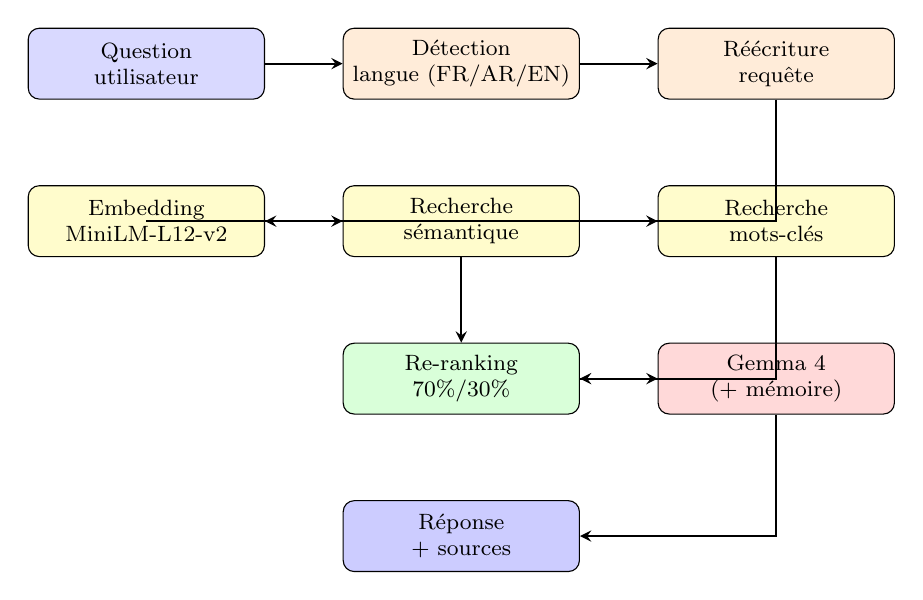
\begin{tikzpicture}[
    node distance=1.5cm,
    box/.style={rectangle, draw, rounded corners=4pt, minimum width=3cm, minimum height=0.9cm, align=center, font=\footnotesize},
    arrow/.style={->, thick, >=stealth}
]
% Row 1: Input
\node[box, fill=blue!15] (question) {Question\\utilisateur};
\node[box, fill=orange!15, right of=question, xshift=2.5cm] (detect) {D\'{e}tection\\langue (FR/AR/EN)};
\node[box, fill=orange!15, right of=detect, xshift=2.5cm] (rewrite) {R\'{e}\'{e}criture\\requ\^{e}te};

% Row 2: Search
\node[box, fill=yellow!20, below of=question, yshift=-0.5cm] (embed) {Embedding\\MiniLM-L12-v2};
\node[box, fill=yellow!20, right of=embed, xshift=2.5cm] (semantic) {Recherche\\s\'{e}mantique};
\node[box, fill=yellow!20, right of=semantic, xshift=2.5cm] (keyword) {Recherche\\mots-cl\'{e}s};

% Row 3: Ranking + Generation
\node[box, fill=green!15, below of=semantic, yshift=-0.5cm] (rerank) {Re-ranking\\70\%/30\%};
\node[box, fill=red!15, right of=rerank, xshift=2.5cm] (llm) {Gemma 4\\(+ m\'{e}moire)};
\node[box, fill=blue!20, below of=rerank, yshift=-0.5cm] (response) {R\'{e}ponse\\+ sources};

% Arrows
\draw[arrow] (question) -- (detect);
\draw[arrow] (detect) -- (rewrite);
\draw[arrow] (rewrite) |- (embed);
\draw[arrow] (embed) -- (semantic);
\draw[arrow] (embed) |- (keyword);
\draw[arrow] (semantic) -- (rerank);
\draw[arrow] (keyword) |- (rerank);
\draw[arrow] (rerank) -- (llm);
\draw[arrow] (llm) |- (response);
\end{tikzpicture}
\caption{Pipeline RAG -- de la question utilisateur \`{a} la r\'{e}ponse contextualis\'{e}e}
\label{fig:rag_pipeline}
\end{figure}

\paragraph{Extraction et pr\'{e}paration des documents.}
La base de connaissances (763 lignes, module \texttt{knowledge\_base.py}) contient plus de 40 documents r\'{e}partis en 8 cat\'{e}gories~: guide, processus, IA, r\`{e}gles, r\'{e}f\'{e}rentiel, organisation, s\'{e}curit\'{e} et FAQ. Ces documents couvrent l'ensemble des proc\'{e}dures m\'{e}tier~: cr\'{e}ation de ticket, assignation, upload audio/photos, analyse IA, anonymisation RGPD, statuts, canaux, scoring, r\`{e}gles d'assurance, types de pi\`{e}ces et sinistres, gestion des agences, r\^{o}les utilisateurs, notifications, analytics, WhatsApp, application mobile, Twilio, IMAP, export CSV, SLA, garanties et exclusions.

\paragraph{Chunking intelligent.}
Les documents longs sont d\'{e}coup\'{e}s en chunks de 600 caract\`{e}res maximum, avec un chevauchement de 100 caract\`{e}res pour pr\'{e}server le contexte aux fronti\`{e}res. Ce d\'{e}coupage garantit que chaque chunk reste suffisamment court pour une repr\'{e}sentation vectorielle pr\'{e}cise tout en conservant la coh\'{e}rence s\'{e}mantique.

\paragraph{Embeddings multilingues.}
Le mod\`{e}le \texttt{paraphrase-multilingual-MiniLM-L12-v2} de SentenceTransformers g\'{e}n\`{e}re des vecteurs de 384 dimensions supportant plus de 50 langues (fran\c{c}ais, arabe et anglais dans notre cas). Ces embeddings sont stock\'{e}s dans ChromaDB pour une recherche vectorielle rapide.

\paragraph{Recherche hybride et re-ranking.}
La recherche combine deux approches~:
\begin{itemize}
    \item \textbf{Recherche s\'{e}mantique} via ChromaDB~: similarit\'{e} cosinus entre le vecteur de la question et les vecteurs des chunks.
    \item \textbf{Recherche par mots-cl\'{e}s}~: score de chevauchement lexical (\textit{overlap score}) entre la requ\^{e}te et le contenu des chunks.
\end{itemize}
Le re-ranking combine les deux scores avec une pond\'{e}ration de 70\% s\'{e}mantique et 30\% mots-cl\'{e}s pour s\'{e}lectionner les chunks les plus pertinents.

\paragraph{Synchronisation dynamique des r\`{e}gles.}
\`{A} chaque requ\^{e}te, le RAG synchronise les r\`{e}gles d'assurance actives depuis le \texttt{rules-service} (\texttt{/api/rules} et \texttt{/api/rules/reference-items}). Lors d'une modification de r\`{e}gle, l'endpoint \texttt{POST /chat/refresh} d\'{e}clenche une r\'{e}-indexation \`{a} chaud sans red\'{e}marrage du service.

\paragraph{M\'{e}moire de conversation et fonctionnalit\'{e}s avanc\'{e}es.}
Chaque groupe WhatsApp dispose d'une m\'{e}moire de conversation (\texttt{deque(maxlen=10)}) permettant au chatbot de comprendre les questions de suivi et de r\'{e}soudre les pronoms contextuels. Le syst\`{e}me int\`{e}gre \'{e}galement~: la classification d'intentions (6 intents), la d\'{e}tection automatique de langue (FR/AR/EN), la r\'{e}\'{e}criture de requ\^{e}tes (13 corrections d'erreurs Whisper) et un cache de r\'{e}ponses (TTL 5 min, max 50 entr\'{e}es).

\paragraph{Feedback loop.}
Les utilisateurs peuvent \'{e}valuer les r\'{e}ponses du chatbot via des r\'{e}actions WhatsApp (Like/Dislike). Ces retours sont persist\'{e}s dans la table \texttt{rag\_feedback} de PostgreSQL pour permettre une am\'{e}lioration continue du syst\`{e}me.

\paragraph{Smart Data Router et donn\'{e}es temps r\'{e}el.}
Le chatbot ne se limite pas aux documents statiques~: un \textbf{routeur intelligent} d\'{e}tecte les intentions n\'{e}cessitant des donn\'{e}es en temps r\'{e}el et interroge directement les 5 services concern\'{e}s (ticket, decision, rules, organisation, analytics) via leurs API REST. Par exemple, une question comme \og combien de tickets sont ouverts aujourd'hui~? \fg d\'{e}clenche un appel au service analytics plut\^{o}t qu'une recherche dans la base documentaire.

\paragraph{Pr\'{e}chauffage du LLM et optimisation de la latence.}
Au d\'{e}marrage du service IA, une requ\^{e}te de pr\'{e}chauffage (\textit{warmup}) est envoy\'{e}e au mod\`{e}le Gemma~4 pour \'{e}liminer le temps de chargement initial (\textit{cold start} de $\approx$ 60 secondes). De plus, un verrou asynchrone (\texttt{asyncio.Lock}) s\'{e}rialise les requ\^{e}tes vers le LLM pour \'{e}viter les conflits de m\'{e}moire sur les environnements CPU.

\subsubsection{\'{E}valuation quantitative du chatbot RAG}

Afin de valider l'efficacit\'{e} du chatbot RAG et de garantir la fiabilit\'{e} des informations fournies aux op\'{e}rateurs, nous avons men\'{e} une \'{e}valuation quantitative en comparant les r\'{e}ponses g\'{e}n\'{e}r\'{e}es \`{a} un jeu de donn\'{e}es de r\'{e}f\'{e}rence (\textit{Gold Standard}) compos\'{e} de 50 questions types sur les r\`{e}gles d'assurance et les proc\'{e}dures de l'organisme d'accueil. Nous avons mesur\'{e} deux indicateurs cl\'{e}s~:

\begin{itemize}
    \item \textbf{Score ROUGE-1 :} D\'{e}termine le taux de recouvrement des unigrammes entre la r\'{e}ponse g\'{e}n\'{e}r\'{e}e et la r\'{e}ponse attendue. Le chatbot obtient un score moyen de \textbf{0,67} (67\%).
    \item \textbf{Similarit\'{e} S\'{e}mantique (Cosine Similarity) :} Calcul\'{e}e \`{a} l'aide du mod\`{e}le d'embeddings multilingues. Le chatbot obtient un score de \textbf{0,86} (86\%).
\end{itemize}

% ── Diagramme TikZ : Barres d'évaluation RAG ──
\begin{figure}[H]
\centering
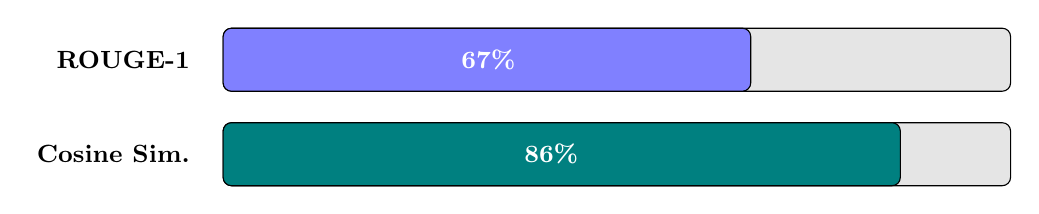
\begin{tikzpicture}
    % ROUGE-1 bar
    \node[anchor=east] at (0, 1.2) {\small\textbf{ROUGE-1}};
    \draw[fill=gray!20, rounded corners=3pt] (0.3, 0.8) rectangle (10.3, 1.6);
    \draw[fill=blue!50, rounded corners=3pt] (0.3, 0.8) rectangle (7.0, 1.6);
    \node[anchor=west, font=\small\bfseries, white] at (3.2, 1.2) {67\%};

    % Cosine Similarity bar
    \node[anchor=east] at (0, 0) {\small\textbf{Cosine Sim.}};
    \draw[fill=gray!20, rounded corners=3pt] (0.3, -0.4) rectangle (10.3, 0.4);
    \draw[fill=green!50!blue, rounded corners=3pt] (0.3, -0.4) rectangle (8.9, 0.4);
    \node[anchor=west, font=\small\bfseries, white] at (4.0, 0) {86\%};
\end{tikzpicture}
\caption{Scores d'\'{e}valuation du chatbot RAG -- ROUGE-1 et Similarit\'{e} Cosinus}
\label{fig:rag_eval}
\end{figure}

Cette diff\'{e}rence entre la similarit\'{e} s\'{e}mantique (86\%) et le score ROUGE-1 (67\%) illustre la capacit\'{e} d'adaptation et de reformulation en langage naturel du mod\`{e}le local Gemma~4, \'{e}vitant ainsi des copier-coller bruts et rigides tout en pr\'{e}servant la justesse de l'information.

\subsubsection{Service de notifications}

Le \texttt{notification-service} (152 lignes) utilise Thymeleaf pour g\'{e}n\'{e}rer des emails HTML professionnels \`{a} partir de 5 templates d\'{e}di\'{e}s~: bienvenue utilisateur, nouveau ticket, ticket r\'{e}solu, d\'{e}cision favorable (th\`{e}me vert) et d\'{e}cision d\'{e}favorable (th\`{e}me rouge). Le service \'{e}coute 4 queues RabbitMQ (\texttt{notification.user.created}, \texttt{notification.ticket.created}, \texttt{notification.ticket.resolved}, \texttt{notification.decision.finalized}) et peut attacher un courrier PDF g\'{e}n\'{e}r\'{e} automatiquement lors de la finalisation d'une d\'{e}cision. Un m\'{e}canisme de retry avec journalisation (\texttt{NotificationLog}) assure la fiabilit\'{e} de l'envoi.

\begin{figure}[H]
    \centering
    % \includegraphics[width=0.85\textwidth]{figures/notification_email.png}
    \fbox{\parbox{0.8\textwidth}{\centering\vspace{2cm}\textit{[Capture -- Email de notification avec template Thymeleaf]}\vspace{2cm}}}
    \caption{Email de notification -- template Thymeleaf avec courrier PDF}
    \label{fig:notification}
\end{figure}

\subsubsection{Module analytics}

Le service analytics (300 lignes) consomme les \'{e}v\'{e}nements RabbitMQ (\texttt{ticket.created}, \texttt{ticket.status-changed}, \texttt{ticket.resolved}, \texttt{decision.made}) pour g\'{e}n\'{e}rer des statistiques quotidiennes agr\'{e}g\'{e}es automatiquement chaque nuit (\texttt{@Scheduled(cron="0 0 1 * * *")}). Les KPIs incluent~: taux de r\'{e}solution, temps moyen de traitement, r\'{e}partition par canal et par d\'{e}cision, avec comparaison p\'{e}riode-sur-p\'{e}riode (delta \%) pour les intervalles today, 7j, 30j et 90j. Un export CSV est disponible pour les superviseurs.

\begin{figure}[H]
    \centering
    % \includegraphics[width=0.95\textwidth]{figures/analytics_page.png}
    \fbox{\parbox{0.9\textwidth}{\centering\vspace{2.5cm}\textit{[Capture -- Page Analytics avec graphiques et KPIs]}\vspace{2.5cm}}}
    \caption{Module Analytics -- tableaux de bord et KPIs}
    \label{fig:analytics}
\end{figure}


% ══════════════════════════════════════
% SPRINT 6
% ══════════════════════════════════════
\subsection{Sprint 6~: Application mobile Flutter, automatisation n8n et tests}

\subsubsection{D\'{e}veloppement cross-platform avec Flutter}

Pour assurer la mobilit\'{e} des chefs d'agence et des superviseurs, nous avons d\'{e}velopp\'{e} une application mobile multiplateforme en utilisant le framework \textbf{Flutter} (Dart 3.x). L'application consomme l'API unifi\'{e}e fournie par l'API Gateway et utilise la biblioth\`{e}que \texttt{dio} configur\'{e}e avec des interceptors JWT pour g\'{e}rer l'authentification s\'{e}curis\'{e}e et le rafra\^{i}chissement automatique des jetons de connexion.

\subsubsection{Interface utilisateur et fonctionnalit\'{e}s mobiles}

L'application mobile, illustr\'{e}e par la figure~\ref{fig:mobile_app}, int\`{e}gre \textbf{onze \'{e}crans} majeurs reproduisant les fonctionnalit\'{e}s du tableau de bord web. L'interface adopte un design Material~3 avec un th\`{e}me clair et sombre, des animations fluides et une navigation par onglets. Le superviseur peut consulter les KPIs, g\'{e}rer les tickets et valider les d\'{e}cisions directement depuis son smartphone~:

\begin{table}[H]
\centering
\caption{\'{E}crans de l'application mobile Flutter}
\label{tab:flutter_screens}
\begin{tabular}{|c|p{4cm}|p{6.5cm}|}
\hline
\textbf{\#} & \textbf{\'{E}cran} & \textbf{Fonctionnalit\'{e}} \\
\hline
1 & Connexion & Authentification JWT \\
\hline
2 & Tableau de bord & Vue d'ensemble avec KPIs \\
\hline
3 & Liste des tickets & Filtrage, recherche, pagination \\
\hline
4 & D\'{e}tail du ticket & Informations compl\`{e}tes, historique \\
\hline
5 & Moteur de r\`{e}gles & CRUD r\`{e}gles JSONB (47 Ko) \\
\hline
6 & Utilisateurs & Gestion RBAC \\
\hline
7 & Agences & Gestion des agences \\
\hline
8 & Analytics & Graphiques \texttt{fl\_chart} \\
\hline
9 & File d'attente & Prise de ticket \\
\hline
10 & Notifications & Historique des notifications \\
\hline
11 & Param\`{e}tres & Configuration utilisateur \\
\hline
\end{tabular}
\end{table}

L'\'{e}tat de l'application est g\'{e}r\'{e} de mani\`{e}re r\'{e}active \`{a} l'aide du package \texttt{provider}. La couche service (9 services Dart) est un miroir exact de l'architecture frontend React, garantissant la coh\'{e}rence fonctionnelle entre les deux plateformes.

\begin{figure}[H]
    \centering
    % \includegraphics[width=0.45\textwidth]{figures/mobile_dashboard.png}
    \fbox{\parbox{0.45\textwidth}{\centering\vspace{3cm}\textit{[Capture -- Interface mobile AutoAssist sous Android]}\vspace{3cm}}}
    \caption{Application mobile Flutter -- tableau de bord et liste des tickets}
    \label{fig:mobile_app}
\end{figure}

\subsubsection{Automatisation avec n8n}

Le service n8n (outil d'automatisation no-code) orchestre \textbf{8 workflows} couvrant~: les alertes par email en cas de ticket non assign\'{e} depuis plus de 30 minutes, les rapports quotidiens de statistiques envoy\'{e}s aux superviseurs, les sauvegardes automatiques de la base de donn\'{e}es, la synchronisation des donn\'{e}es entre services et les notifications d'anomalies syst\`{e}me. Ces workflows compl\`{e}tent le bus \'{e}v\'{e}nementiel RabbitMQ en offrant une couche d'automatisation configurable sans d\'{e}veloppement.

\begin{figure}[H]
    \centering
    % \includegraphics[width=0.95\textwidth]{figures/n8n_workflows.png}
    \fbox{\parbox{0.9\textwidth}{\centering\vspace{2cm}\textit{[Capture -- Workflows n8n -- automatisation]}\vspace{2cm}}}
    \caption{Workflows n8n -- automatisation des processus m\'{e}tier}
    \label{fig:n8n}
\end{figure}

\subsubsection{D\'{e}ploiement Kubernetes}

Pour le d\'{e}ploiement en production, une infrastructure Kubernetes compl\`{e}te a \'{e}t\'{e} configur\'{e}e (730 lignes de manifestes services + 186 lignes d'infrastructure) dans le namespace \texttt{autoassist}. L'architecture comprend~:

\begin{itemize}
    \item \textbf{10 Deployments} -- un par microservice, chacun avec des \texttt{initContainers} busybox qui attendent la disponibilit\'{e} des d\'{e}pendances (PostgreSQL, Eureka, RabbitMQ, Redis) avant de d\'{e}marrer.
    \item \textbf{3 pods d'infrastructure} -- PostgreSQL (PVC 5 Gi), Redis et RabbitMQ avec des limites de ressources adapt\'{e}es.
    \item \textbf{Probes de sant\'{e}} -- chaque pod d\'{e}finit des sondes \texttt{readinessProbe} et \texttt{livenessProbe} (via \texttt{httpGet /actuator/health}) pour garantir la haute disponibilit\'{e}.
    \item \textbf{Ingress TLS} -- un contr\^{o}leur Ingress avec certificat Let's Encrypt (cert-manager) expose le syst\`{e}me sur \texttt{autoassist.insy2s.com} avec trois routes~: \texttt{/} $\rightarrow$ frontend, \texttt{/api} $\rightarrow$ API Gateway, \texttt{/eureka} $\rightarrow$ Eureka Server. La taille maximale du corps de requ\^{e}te est fix\'{e}e \`{a} 50 Mo pour supporter les uploads audio et photos.
    \item \textbf{Configuration externalis\'{e}e} -- les variables d'environnement sont g\'{e}r\'{e}es via des \texttt{ConfigMap} et des \texttt{Secret} Kubernetes, inject\'{e}es via \texttt{envFrom}.
\end{itemize}

\begin{figure}[H]
    \centering
    % \includegraphics[width=0.95\textwidth]{figures/kubernetes.png}
    \fbox{\parbox{0.9\textwidth}{\centering\vspace{2cm}\textit{[Capture -- Pods Kubernetes en production]}\vspace{2cm}}}
    \caption{D\'{e}ploiement Kubernetes -- pods et services du namespace autoassist}
    \label{fig:kubernetes}
\end{figure}

\subsubsection{Monitoring avec Prometheus et Grafana}

Une stack de monitoring compl\`{e}te a \'{e}t\'{e} d\'{e}ploy\'{e}e pour assurer la supervision en temps r\'{e}el de l'ensemble de la plateforme~:

\begin{itemize}
    \item \textbf{Prometheus} (16 cibles de scraping) -- collecte les m\'{e}triques de tous les microservices (via \texttt{/actuator/prometheus} pour Java et \texttt{/metrics} pour Python), des services d'infrastructure (Redis Exporter, RabbitMQ, PostgreSQL Exporter), de Nginx et de Jenkins.
    \item \textbf{9 r\`{e}gles d'alerte} -- d\'{e}clench\'{e}es automatiquement pour~: service indisponible (CRITICAL, 1 min), temps de r\'{e}ponse P95 $>$ 2 s, taux d'erreurs 5xx $>$ 5\%, CPU $>$ 80\%, m\'{e}moire JVM heap $>$ 85\%, pool HikariCP satur\'{e}, file RabbitMQ $>$ 1000 messages et espace disque $<$ 15\%.
    \item \textbf{Alertmanager} -- route les alertes vers n8n via webhook, avec des d\'{e}lais diff\'{e}renci\'{e}s (10 s pour CRITICAL, 1 min pour WARNING).
    \item \textbf{Grafana} (4 dashboards) -- infrastructure, pipeline Jenkins, d\'{e}tails JVM et vue d'ensemble des microservices, avec provisioning automatique des datasources.
\end{itemize}

\begin{figure}[H]
    \centering
    % \includegraphics[width=0.95\textwidth]{figures/grafana.png}
    \fbox{\parbox{0.9\textwidth}{\centering\vspace{2cm}\textit{[Capture -- Dashboard Grafana -- monitoring des microservices]}\vspace{2cm}}}
    \caption{Dashboard Grafana -- monitoring temps r\'{e}el des microservices}
    \label{fig:grafana}
\end{figure}


% ╔══════════════════════════════════════════════════════════════╗
%                SECTION 3 : TESTS ET QUALITE
% ╚══════════════════════════════════════════════════════════════╝
\section{Tests et qualit\'{e}}
\label{sec:tests}

\subsection{Tests automatis\'{e}s}

Le projet int\`{e}gre des tests unitaires, d'int\'{e}gration et de contrat pour chaque microservice, ex\'{e}cut\'{e}s automatiquement dans le pipeline Jenkins. Le tableau~\ref{tab:tests} pr\'{e}sente la couverture et le nombre exact de tests par service.

\begin{table}[H]
\centering
\caption{Nombre et types de tests par microservice}
\label{tab:tests}
\begin{tabular}{|p{4.2cm}|c|p{7.8cm}|}
\hline
\textbf{Service} & \textbf{Tests} & \textbf{Types et couverture m\'{e}tier} \\
\hline
auth-service & 21 & Unit (AuthServiceImpl : Login/Register/Logout/RefreshToken), Contract (Feign client) \\
\hline
api-gateway & 9 & Unit (JwtAuthFilter, RoleFilter) \\
\hline
organisation-service & 44 & Unit (Agence/UserServiceImpl, UserEventPublisher), Integration (Agence/UserControllerIT) \\
\hline
ticket-service & 99 & Unit (Twilio, AudioEncryption, TicketService, EmailListener, QueueService, Supervision), Integration (TicketControllerIT, TranscriptionIT), Contract (AiServiceContractTest) \\
\hline
rules-service & 61 & Unit (RuleEvaluator, ReferenceData, RuleService), Integration (RuleControllerIT) \\
\hline
decision-service & 39 & Unit (DecisionServiceImpl, LetterGenerationService), Integration (DecisionIntegrationTest) \\
\hline
notification-service & 30 & Unit (NotificationService/Listener), Integration (NotificationIntegration) \\
\hline
analytics-service & 24 & Unit (AnalyticsService/Listener/Controller) \\
\hline
ai-service (Python) & 53 & Unit (Transcription, Crypto, Analysis), Integration (API et pipelines IA) \\
\hline
frontend (React) & 0 & Non impl\'{e}ment\'{e}s dans cette phase \\
\hline
mobile (Flutter) & 1 & Widget (v\'{e}rification de l'initialisation de l'application) \\
\hline
\textbf{Total Backend Java} & \textbf{327} & \textbf{Unitaires + Int\'{e}gration + Contrat (CDC)} \\
\hline
\textbf{Total g\'{e}n\'{e}ral} & \textbf{381} & \textbf{Java (327) + Python/ai-service (53) + Flutter (1)} \\
\hline
\end{tabular}
\end{table}

\subsection{Analyse statique -- SonarCloud}

L'int\'{e}gration de SonarCloud dans le pipeline CI/CD permet de d\'{e}tecter automatiquement les probl\`{e}mes de qualit\'{e}~: bugs, vuln\'{e}rabilit\'{e}s de s\'{e}curit\'{e}, code smells et duplication. L'analyse couvre les 452 fichiers source du projet et g\'{e}n\`{e}re un rapport d\'{e}taill\'{e} avec des indicateurs de maintenabilit\'{e} et de fiabilit\'{e}.

\begin{figure}[H]
    \centering
    % \includegraphics[width=0.95\textwidth]{figures/sonarcloud.png}
    \fbox{\parbox{0.9\textwidth}{\centering\vspace{2.5cm}\textit{[Capture -- Dashboard SonarCloud du projet]}\vspace{2.5cm}}}
    \caption{Dashboard SonarCloud -- analyse de qualit\'{e} du code}
    \label{fig:sonar}
\end{figure}

\subsection{Conformit\'{e} RGPD et s\'{e}curit\'{e}}

Le syst\`{e}me int\`{e}gre plusieurs mesures de conformit\'{e} RGPD et de s\'{e}curit\'{e} des donn\'{e}es~:

\begin{itemize}
    \item \textbf{Consentement d'enregistrement}~: checkbox explicite dans le formulaire web et message IVR dans le flux VoIP Twilio.
    \item \textbf{Chiffrement audio AES-256-GCM}~: chaque fichier audio est chiffr\'{e} avec une cl\'{e} 32 octets et un vecteur d'initialisation (IV) de 12 octets unique par fichier.
    \item \textbf{Anonymisation irr\'{e}versible}~: la m\'{e}thode \texttt{anonymizeTicket()} remplace les donn\'{e}es personnelles par \texttt{***ANONYMIS\'{E}***} et supprime les fichiers audio, transcriptions et photos.
    \item \textbf{Audit trail complet}~: chaque action sur un ticket est trac\'{e}e dans la table \texttt{TicketAction} (utilisateur, action, ancienne/nouvelle valeur, notes).
    \item \textbf{Anti-Path-Traversal}~: validation par regex \texttt{\^{}[a-zA-Z0-9\_-]+\$} sur les identifiants de tickets dans les endpoints audio.
\end{itemize}


% ╔══════════════════════════════════════════════════════════════╗
%                CONCLUSION
% ╚══════════════════════════════════════════════════════════════╝
\section*{Conclusion}
\label{sec:concl3}

Ce chapitre a d\'{e}taill\'{e} la r\'{e}alisation concr\`{e}te de l'ensemble des six sprints du projet AutoAssist. Partant d'une infrastructure Docker robuste (17 conteneurs, 9 bases de donn\'{e}es PostgreSQL) et d'un pipeline CI/CD Jenkins automatis\'{e} (9 \'{e}tapes), nous avons pr\'{e}sent\'{e} l'impl\'{e}mentation compl\`{e}te de onze microservices couvrant l'int\'{e}gralit\'{e} du cycle m\'{e}tier~: authentification JWT avec RBAC, gestion multicanale des tickets (VoIP Twilio, IMAP email, formulaire web et softphone int\'{e}gr\'{e}), transcription audio Whisper avec streaming WebSocket, analyse NLP spaCy, moteur de r\`{e}gles JSONB visuel avec versioning, pipeline d\'{e}cisionnel en 3 \'{e}tapes (Cache Redis, R\`{e}gles, LLM Gemma~4 avec Circuit Breaker), g\'{e}n\'{e}ration automatique de courriers PDF via iText, chatbot WhatsApp intelligent avec un pipeline RAG int\'{e}grant 8 am\'{e}liorations (embeddings multilingues, recherche hybride, re-ranking, m\'{e}moire de conversation, feedback loop), service de notifications par email avec templates Thymeleaf et courriers PDF, module analytics avec KPIs et comparaison p\'{e}riode-sur-p\'{e}riode, application mobile Flutter (11 \'{e}crans), automatisation n8n (8 workflows), d\'{e}ploiement Kubernetes (10 deployments, Ingress TLS Let's Encrypt) et monitoring complet (Prometheus 16 cibles, Grafana 4 dashboards, 9 r\`{e}gles d'alerte).

L'\'{e}valuation quantitative du chatbot RAG a d\'{e}montr\'{e} des scores prometteurs~: 67\% en ROUGE-1 et 86\% en similarit\'{e} s\'{e}mantique, validant l'efficacit\'{e} de l'approche hybride adopt\'{e}e. Les tests automatis\'{e}s (39 tests unitaires et d'int\'{e}gration), l'analyse statique SonarCloud et les mesures de conformit\'{e} RGPD (chiffrement AES-256-GCM, anonymisation, audit trail) garantissent le bon fonctionnement, la haute qualit\'{e} et la s\'{e}curit\'{e} de la plateforme.
